\documentclass[11pt,a4paper]{article}
\usepackage{gtu-el-yazisi}
\begin{document}
\notbilgi{Alan Teorisi}{Ders 14 -- Görüntü kavramı ve yöntemi}{Ders14.pdf}

\sayfa{1}
\section{Görüntü kavramı ve yöntemi}

\begin{center}
\begin{tikzpicture}[line width=0.8pt]
  \draw[-{Stealth}] (0,-1.9) -- (0,3.4) node[right] {$z$};
  \draw (-3.6,0) -- (3.4,0);
  \draw[-{Stealth}] (3.3,0) -- (3.6,0) node[right] {$z=0$};
  \foreach \hx in {-3.4,-2.95,...,-0.4,0.4,0.85,...,3.0} \draw (\hx,0) -- ++(-0.1,-0.2);
  \node at (-3.1,2.3) {(I)};
  \node at (-1.3,1.5) {$\varepsilon_1$};
  \node at (-3.1,-1.3) {(II)};
  \node at (-1.3,-1.0) {$\varepsilon_2$};
  \node at (-3.3,0.4) {$z=0$};
  \node[anchor=east,align=right] at (-3.7,-0.25) {$v=0$\\[-1pt]$z=0$};
  \fill (1.8,2.0) circle (1.3pt);
  \node[anchor=west] at (1.85,2.0) {$q$};
  \node at (2.3,2.8) {$P(x,y,z)$};
  \node[turuncukalem] at (1.7,1.0) {$\vec D_1\neq 0$};
  \node[turuncukalem] (rs) at (3.6,1.1) {$\rho_s\neq 0$};
  \draw[turuncukalem,-{Stealth}] (rs.south west) -- (2.9,0.1);
  \node[turuncukalem] at (1.5,-1.0) {$\vec D_2=0$};
\end{tikzpicture}
\end{center}

\begin{align*}
\rho_s &= \vec e_z\bigl(\vec D_1-\underbrace{\vec D_2}_{0}\bigr)\Big|_{z=0} \\
&= \vec e_z\,\vec D_1\Big|_{z=0} = -\vec e_z\,\varepsilon_1\,\mathrm{grad}\,V_1\Big|_{z=0}
\end{align*}

$z<0$ bölgesi ($\varepsilon_2$ dielektrik sabitli bölge)

\noindent
\begin{minipage}[t]{0.38\linewidth}
$V_2=0$ sabit

$\vec E_2=0$ ; $\vec D_2=0$
\end{minipage}\hfill
\begin{minipage}[t]{0.58\linewidth}
II nolu bölgede yük olmadığından ve $z=0$ yüzeyi üzerinde $v=0$ sabit olduğundan bölge iletkendir ve potansiyeli $V_2=0$ olur.
\end{minipage}

$z>0$ bölgesi ($\varepsilon_1$ dielektrik sabitli bölge)

$V_1=\,?$ \quad $\vec E=-\mathrm{grad}\,V_1$ ; \quad $\vec D_1=\varepsilon_1\vec E_1=-\varepsilon_1\,\mathrm{grad}\,V_1$

$z>0$ bölgesinin $\rho=q\,\delta(x-x_0)\,\delta(y-y_0)\,\delta(z-z_0)\neq 0$

I nolu bölge ise II gibi iletken bir bölgede değil, $V_1\neq 0$

(I) $V_1$'in sağladığı diferansiyel denklem ve sınır koşul dikkate alınmalı.

\[
\text{$z>0$ da}\quad
\begin{cases}
\Delta V_1=-\dfrac{\rho}{\varepsilon_1}=-\dfrac{q\,\delta(x-x_0)\,\delta(y-y_0)\,\delta(z-z_0)}{\varepsilon_1} \\[3mm]
V_1\big|_{z=0}=0 \qquad \displaystyle\lim_{z\to\infty}V_1 \text{ için } <\infty
\end{cases}
\]

\medskip
Ek örnek problem

\begin{center}
\begin{tikzpicture}[line width=0.8pt]
  \draw (0,-1.7) -- (0,2.7);
  \draw[dashed] (-3.6,0) -- (4.2,0);
  \node[align=left] at (-3.3,1.3) {yüzey\\[-2pt]yerine\\[-2pt]yük koyduk};
  \node at (-3.9,0) {$\equiv$};
  \node at (-1.7,0.45) {$\varepsilon_1$};
  \node at (-1.7,-0.9) {$\varepsilon_2$};
  \fill (2.0,2.1) circle (1.3pt);
  \node[anchor=north west] at (2.0,2.1) {$q$};
  \node at (3.4,2.5) {$P_0(x_0,y_0,z_0)$};
  \node[anchor=west] at (4.3,0) {$\rho_s\quad V=0$};
\end{tikzpicture}
\end{center}

\sayfa{2}
\begin{center}
\begin{tikzpicture}[line width=0.8pt]
  \node[anchor=west] at (-3.2,2.8) {$z>0$ bölgesi bakımından};
  \node[anchor=west] at (-2.4,2.2) {bir birine özdeştir};
  % sol sekil
  \draw (0,-1.95) -- (0,1.95);
  \draw (-2.6,0) -- (1.9,0);
  \foreach \hx in {-2.2,-1.8,...,1.7} \draw (\hx,0) -- ++(-0.1,-0.25);
  \node at (-1.25,1.0) {$\varepsilon_1$};
  \node at (-1.3,-1.0) {$\varepsilon_2$};
  \fill (1.2,1.25) circle (1pt);
  \node[anchor=west] at (1.3,1.2) {$q$};
  \node at (2.35,0) {$\equiv$};
  % sag sekil
  \node[kirmizikalem,align=center] at (6.6,2.5) {altı baştan biliyoruz\\yukarısı özdeştir};
  \begin{scope}[shift={(5.8,0)}]
    \draw (0,-1.35) -- (0,1.9);
    \draw (-3.05,0) -- (3.2,0);
    \node at (-1.6,0.67) {$\varepsilon_1$};
    \node at (-1.75,-0.57) {$\varepsilon_1$};
    \draw[dashed] (1.4,0.81) -- (1.38,-0.70);
    \fill (1.4,0.81) circle (1pt);
    \fill (1.38,-0.70) circle (1pt);
    \node[anchor=west] at (1.55,0.8) {$q$};
    \node[anchor=west] at (1.5,-0.72) {$-q$};
    \draw[kirmizikalem,dashed] (0,0) -- (1.4,0.81);
    \node[kirmizikalem] at (0.65,0.7) {$r_1$};
    \draw[kirmizikalem] (0,-0.05) -- (1.38,-0.05);
    \node[kirmizikalem] at (0.8,-0.27) {$\ell$};
    \draw[turuncukalem,dashed] (0,0) -- (1.38,-0.70);
    \node[turuncukalem] at (0.6,-0.65) {$r_2$};
    \node at (3.5,-0.5) {$z=0$};
    \node at (2.9,1.3) {$P_0(x_0,y_0,z_0)$};
    \draw[-{Stealth}] (1.7,-1.2) -- (1.62,-0.9);
    \node at (3.0,-1.5) {$P_1(x_0,y_0,-z_0)$};
  \end{scope}
  % buyuk ok
  \draw (2.76,-0.9) .. controls (3.2,-2.7) and (4.5,-3.2) .. (7.0,-3.15) .. controls (8.8,-3.1) and (9.7,-2.7) .. (9.9,-2.15);
  \draw[-{Stealth}] (3.8,-2.2) .. controls (0.5,-2.6) and (-2.4,-2.2) .. (-2.95,-2.9) .. controls (-3.3,-3.3) and (-3.2,-3.6) .. (-3.1,-3.85);
\end{tikzpicture}
\end{center}

\[
z>0\ \text{da}\quad \Delta V_1=-\frac{\rho_1}{\varepsilon_1}=-\frac{q\,\delta(x-x_0)\,\delta(y-y_0)\,\delta(z-z_0)}{\varepsilon_1}
\]
\[
V_q\Big|_{z=0}=\frac{q}{4\pi\varepsilon_1 r_1}\qquad\qquad V_{-q}\Big|_{z=0}=\frac{-q}{4\pi\varepsilon_1 r_2}
\]

\noindent
\begin{minipage}[c]{0.40\linewidth}
$r_1=r_2=\sqrt{z_0^{\,2}+\ell^{2}}$
\end{minipage}\hfill
\begin{minipage}[c]{0.56\linewidth}
\textcolor{kirmizikalem}{* Tüm uzay homojense Coulomb yasası geçerli}
\end{minipage}

\begin{align*}
V\Big|_{z=0} &= V_q\Big|_{z=0}+V_{-q}\Big|_{z=0} \\
&= \frac{q}{4\pi\varepsilon_1 r_1}-\frac{q}{4\pi\varepsilon_1 r_1}=V_1\Big|_{z=0}=0
\end{align*}

\begin{center}
\begin{tikzpicture}[line width=0.8pt]
  \draw[{Stealth}-{Stealth}] (0,-1.55) -- (0,2.15);
  \draw[-{Stealth}] (-2.55,0) -- (4.0,0);
  \draw (-1.28,0.6) -- (1.88,0.6);
  \draw (-1.28,0.6) -- (1.9,-0.62);
  \draw[kirmizikalem] (-1.35,-0.04) -- (1.88,0.6);
  \draw[turuncukalem] (-1.35,-0.06) -- (1.9,-0.62);
  \fill (-1.28,0.6) circle (1.3pt);
  \fill (1.88,0.6) circle (1.3pt);
  \fill (1.9,-0.62) circle (1.3pt);
  \node at (-1.4,0.95) {$P$};
  \node[anchor=west] at (2.0,0.65) {$q$};
  \node[anchor=west] at (2.05,-0.65) {$-q$};
  \node at (0.9,0.85) {$r_1$};
  \node at (1.0,-0.55) {$r_2$};
  \node at (-2.0,0.35) {$\varepsilon_1$};
  \node at (-1.75,-0.85) {$\varepsilon_1$};
  \node[kirmizikalem,font=\small] at (0.85,0.28) {$r_1|_{z=0}$};
  \node[turuncukalem,font=\small] at (-0.15,-0.5) {$r_2|_{z=0}$};
\end{tikzpicture}
\end{center}

\[ V_P=\frac{q}{4\pi\varepsilon_1 r_1}-\frac{q}{4\pi\varepsilon_1 r_2} \]
\[ V_P=\frac{q}{4\pi\varepsilon_1}\left(\frac{1}{r_1}-\frac{1}{r_2}\right) \]
\[ V_1\Big|_{z=0}=V_P\Big|_{z=0}=\frac{q}{4\pi\varepsilon_1}\left(\frac{1}{r_1\big|_{z=0}}-\frac{1}{r_2\big|_{z=0}}\right)=0 \]

\sayfa{3}
\begin{align*}
\Rightarrow\ z>0\quad & V_1=\frac{q}{4\pi\varepsilon_1}\left(\frac{1}{r_1}-\frac{1}{r_2}\right) \\
z<0\quad & V_2=0
\end{align*}

\begin{align*}
\Rightarrow\ \vec E_1=-\mathrm{grad}\,V_1 &= \frac{q}{4\pi\varepsilon_1}\,\frac{\vec r_1}{r_1^{3}}-\frac{q}{4\pi\varepsilon_1}\,\frac{\vec r_2}{r_2^{3}} \\
\vec D_1=\varepsilon_1\vec E_1 &= \frac{q}{4\pi}\left(\frac{\vec r_1}{r_1^{2}}-\frac{\vec r_2}{r_2^{3}}\right)\qquad\text{\footnotemark}
\end{align*}
\footnotetext{Claude notu: muhtemelen $r_1^{3}$ olmalı.}

\[ \rho_s\Big|_{z=0}=\vec e_z\bigl(\vec D_1-\vec D_2\bigr)\Big|_{z=0}=\vec e_z\cdot\vec D_1\Big|_{z=0} \]
\[ \rho_s=\frac{q}{4\pi}\,\vec e_z\left(\frac{\vec r_1}{r_1^{3}}\Big|_{z=0}-\frac{\vec r_2}{r_2^{3}}\right)\Big|_{z=0} \]

\begin{center}
\begin{tikzpicture}[line width=0.8pt]
  \draw[-{Stealth}] (-3.0,0) -- (4.5,0);
  \draw[{Stealth}-{Stealth}] (0,-1.75) -- (0,2.5);
  \draw[kirmizikalem,line width=1pt] (-1.57,-0.05) -- (2.11,0.69);
  \draw[turuncukalem,line width=1pt] (-1.57,-0.06) -- (2.14,-0.71);
  \fill (2.11,0.69) circle (1.2pt);
  \fill (2.14,-0.71) circle (1.2pt);
  \node[anchor=west] at (2.2,0.7) {$q$};
  \node[anchor=west] at (2.25,-0.72) {$-q$};
  \draw[morkalem,-{Stealth}] (-1.57,-0.05) -- (-2.14,0.42);
  \node[morkalem] at (-1.55,0.5) {$\vec r_2$};
  \draw[murekkep,-{Stealth}] (-1.57,-0.06) -- (-2.33,-0.42);
  \node[murekkep] at (-1.9,-0.62) {$\vec r_1$};
  \node[kirmizikalem] at (-0.45,0.62) {$\vec r_1$};
  \node[turuncukalem] at (0.35,-0.78) {$\vec r_2$};
  \node at (0.95,0.95) {$r_1$};
  \node at (1.05,-0.62) {$r_2$};
  \node at (-2.7,0.45) {$\varepsilon_1$};
  \node at (-2.0,-1.0) {$\varepsilon_1$};
  \node[murekkep,font=\small] at (-0.22,0.14) {$\theta$};
  \node[morkalem,font=\small] at (-0.22,-0.17) {$\theta$};
  \node[morkalem,font=\small] at (-2.05,0.14) {$\theta$};
  \node[murekkep,font=\small] at (-2.15,-0.14) {$\theta$};
  \node[turuncukalem] at (2.0,-1.4) {$|\vec r_1|=|\vec r_2|$};
  \node[turuncukalem] at (2.15,-2.0) {$\vec r_1\neq\vec r_2$};
  \node at (6.6,1.6) {$\vec r_1\big|_{z=0}=r_1\cdot\vec n_1$};
\end{tikzpicture}
\end{center}

\[ \vec r_1=r_1\Big|_{z=0}\,n_1\Big|_{z=0}=r_1\bigl[\cos\theta\,\vec e_z-\sin\theta\,\vec e_z\bigr]\qquad\text{\footnotemark} \]
\footnotetext{Claude notu: $\cos\theta$ ile çarpılan birim vektör muhtemelen düzlem içi yöndeki birim vektör olmalı ($\vec e_z$ değil); $\sin\theta$ ile çarpılan ise $\vec e_z$. Aşağıdaki satırlar için de aynı.}
{\color{morkalem}\[ \vec r_2\Big|_{z=0}=r_2\Big|_{z=0}\,n_2\Big|_{z=0}=r_2\bigl[\cos\theta\,\vec e_z+\sin\theta\,\vec e_z\bigr] \]}
\[ r_1=r_2=r \]

\begin{align*}
\Rightarrow\ \rho_s &= \frac{q}{4\pi}\,\vec e_z\left(\frac{\vec r_1\big|_{z=0}}{\underbrace{\bigl(r_1\big|_{z=0}\bigr)^{3}}_{r^3}}-\frac{\vec r_2\big|_{z=0}}{\underbrace{\bigl(r_2\big|_{z=0}\bigr)^{3}}_{r^3}}\right) \\
&= \frac{q}{4\pi}\,\frac{\vec e_z}{r^{3}}\left(\vec r_1\big|_{z=0}-\vec r_2\big|_{z=0}\right) \\
&= \frac{q}{4\pi r^{3}}\,\vec e_z\Bigl[\,r\cos\theta\,\vec e_z-r\sin\theta\,\vec e_z-r\cos\theta\,\vec e_\ell-r\sin\theta\,\vec e_z\Bigr] \\
&= \frac{-q\sin\theta}{2\pi r^{2}} \qquad \text{ve}\ \sin\theta=\frac{\text{Karşı}}{\text{hipo}}=\frac{z_0}{r}
\intertext{\hfill\textcolor{kirmizikalem}{yüzeyin üzerindeki yük 0 değildir ve değişkendir}}
&= \frac{-q\,z_0}{2\pi r^{3}} \qquad (\mathrm{C/m^{2}})
\end{align*}

\sayfa{4}
\newcommand\kadran[2]{%
\begin{scope}[shift={(#1,#2)}]
  \draw[{Stealth}-{Stealth}] (0,-1.7) -- (0,2.25);
  \draw[-{Stealth}] (-2.7,0) -- (3.0,0);
  \node at (3.3,-0.05) {$\rho_s$};
  \foreach \hy in {0.5,0.9,1.3,1.7,2.0} \draw (0,\hy) -- ++(-0.08,0.16);
  \foreach \hx in {0.4,0.9,...,2.7} \draw (\hx,0) -- ++(-0.08,-0.14);
  \draw (-1.35,1.45) -- (1.5,1.5);
  \fill (-1.45,1.5) circle (1pt); \node at (-1.5,1.85) {$-q$};
  \fill (1.6,1.52) circle (1pt); \node[anchor=west] at (1.7,1.55) {$q$};
  \fill (-1.48,-1.5) circle (1pt); \node at (-1.85,-1.8) {$q$};
  \fill (1.55,-1.55) circle (1pt); \node[anchor=west] at (1.7,-1.68) {$-q$};
  \draw[turuncukalem] (0.0,0.32) -- (0.67,1.8);
  \draw[turuncukalem] (0.6,0.15) -- (1.35,1.62);
  \draw[turuncukalem] (1.15,0.22) -- (1.8,1.42);
  \draw[turuncukalem] (1.65,0.12) -- (2.25,1.22);
\end{scope}}
\begin{center}
\begin{tikzpicture}[line width=0.7pt,x=0.9cm,y=0.9cm]
  \kadran{0}{0}
  \kadran{9.17}{-0.18}
  \node at (1.2,1.15) {$\varepsilon_1$};
  \node at (5.05,0.2) {$\equiv$};
  \node at (10.45,1.1) {$\varepsilon_1$};
  \node at (7.85,0.55) {$\varepsilon_1$};
  \node at (7.95,-1.05) {$\varepsilon_1$};
  \node at (10.4,-1.1) {$\varepsilon_1$};
  \draw (2.3,1.0) .. controls (4.5,2.3) and (7.0,2.6) .. (9.2,1.3);
  \draw[-{Stealth}] (6.05,2.15) -- (6.05,1.7);
  \node at (6.5,1.3) {bu bölgede};
\end{tikzpicture}
\end{center}

\begin{center}
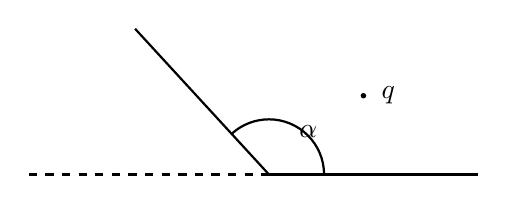
\begin{tikzpicture}[line width=0.8pt]
  \draw[dashed] (-3.05,0) -- (0,0);
  \draw (0,0) -- (2.65,0);
  \draw (0,0) -- (-1.7,1.85);
  \draw (0.7,0) arc (0:132:0.7);
  \node at (0.5,0.55) {$\alpha$};
  \fill (1.2,1.0) circle (1pt);
  \node[anchor=west] at (1.3,1.0) {$q$};
\end{tikzpicture}
\end{center}

\[ n_i=\frac{2\pi}{\alpha}-1 \qquad \text{görüntü yük sayısı} \]
tam sayı gelmezse sonsuz görüntü var demektir.

\bigskip
\begin{center}
\begin{tikzpicture}[line width=0.7pt,x=0.8cm,y=0.8cm]
  \draw[-{Stealth}] (0,-1.26) -- (0,1.67) node[right=2pt] {$z$};
  \draw[-{Stealth}] (-2.07,0) -- (2.23,0) node[right=2pt] {$z=0$};
  \foreach \hx in {-2.0,-1.75,...,-0.25} \draw (\hx,0) -- ++(-0.07,-0.13);
  \foreach \hx in {0.5,0.75,...,1.75} \draw (\hx,0) -- ++(-0.07,-0.13);
  \node at (-1.62,1.24) {(I)};
  \node at (-0.57,0.77) {$\varepsilon_1$};
  \node at (-1.4,-1.05) {(II)};
  \node at (-0.6,-0.58) {$\varepsilon_2$};
  \fill (1.26,0.84) circle (1pt);
  \node[anchor=west] at (1.3,0.84) {$q$};
  \node at (2.0,1.3) {$P(x,y,z)$};
  \node[turuncukalem] at (1.55,0.4) {$\vec D_1\neq 0$};
  \node[turuncukalem] at (3.5,0.55) {$\rho_s\neq 0$};
  \draw[turuncukalem,-{Stealth}] (2.1,0.05) -- (2.55,0.4);
  \node[turuncukalem] at (1.28,-0.56) {$\vec D_2=0$};
  \node at (-1.9,0.3) {$z=0$};
  \node at (-2.5,-0.7) {$V=V_s$};
  \node at (4.4,0) {$\equiv$};
  \begin{scope}[shift={(7.3,-0.1)}]
    \draw (0,-1.36) -- (0,1.59);
    \draw (-2.35,0) -- (1.22,0);
    \node at (-0.9,0.62) {$\varepsilon_1$};
    \node at (0.5,0.62) {$V_s$};
    \node at (-2.02,0.2) {$V_s$};
    \node at (-0.95,-0.63) {$\varepsilon_2$};
    \node at (0.75,-0.56) {$V_s$};
  \end{scope}
  \node at (9.0,0) {$+$};
  \begin{scope}[shift={(11.1,0)}]
    \draw (0,-1.23) -- (0,1.49);
    \draw (-1.8,0) -- (1.85,0);
    \foreach \hx in {-1.5,-1.2,...,-0.3} \draw (\hx,0) -- ++(-0.07,-0.13);
    \foreach \hx in {0.3,0.6,...,1.5} \draw (\hx,0) -- ++(-0.07,-0.13);
    \node at (-0.65,1.14) {$\varepsilon_1$};
    \fill (0.7,0.99) circle (1pt);
    \node[anchor=west] at (0.75,1.0) {$q$};
    \node[anchor=west] at (1.95,0.2) {$v=0$};
    \node at (0.9,-0.61) {$\varepsilon_2$};
  \end{scope}
\end{tikzpicture}
\end{center}

\begin{center}
\begin{tikzpicture}[line width=0.8pt]
  \fill (0,0) circle (1pt);
  \node at (0.1,-0.3) {$q_1$};
  \draw[dashed] (0,0) -- (2.88,2.52);
  \fill (2.88,2.52) circle (1pt);
  \node[anchor=west] at (2.95,2.55) {$q_2$};
  \fill (1.68,1.49) circle (1pt);
  \node at (1.5,1.95) {$P$};
  \node at (0.68,1.02) {$r$};
  \fill (-1.02,1.47) circle (1pt);
  \node at (-1.4,1.15) {$q_3$};
  \node[anchor=west] at (2.15,1.2) {$V=\dfrac{q_1}{4\pi\varepsilon r}$};
  \node[anchor=west,align=left] at (6.0,2.2) {$q_1$ baştan vardı\\[1mm]$q_2$ uzaktan getirildi};
\end{tikzpicture}
\end{center}

\[ W=q_2\bigl(V_1-\underbrace{V_\infty}_{0}\bigr)=q_2\,\frac{q_1}{4\pi\varepsilon r} \]

\begin{align*}
W &= \frac{1}{2}\sum_{i=1}^{n} q_i V_i \\
&= \frac{1}{2}\bigl[\,q_1V_1+q_2V_2+\cdots+q_nV_n\bigr]
\end{align*}

\begin{align*}
W_1 &= W_{13}+W_{23}+W_{12} \\
&= \frac{q_3 q_1}{4\pi\varepsilon r_{13}}+\frac{q_3\cdot q_2}{4\pi\varepsilon r_{23}}+\frac{q_1\cdot q_2}{4\pi\varepsilon r_{12}}
\end{align*}

\sayfa{5}
\begin{center}
\begin{tikzpicture}[line width=0.7pt]
  \node at (0,0) {$\times$};
  \node at (2.42,0.67) {$\times$};
  \node at (4.37,-0.5) {$\times$};
  \node at (3.3,-1.62) {$\times$};
  \fill (5.55,0.37) circle (0.8pt);
  \node at (0.15,0.32) {$q_1$};
  \node at (0.45,0.9) {$V_1$};
  \node[anchor=west] at (2.55,0.8) {$q_2$};
  \node at (3.2,1.3) {$V_2$};
  \node[anchor=west] at (4.5,-0.5) {$q_3$};
  \node at (4.7,0.05) {$V_3$};
  \node at (3.4,-2.0) {$q_n$};
  \node at (3.0,-1.25) {$V_4$};
  \node[anchor=west] at (5.65,0.35) {$q_i$};
  \node at (6.3,0.85) {$V_i$};
  \draw[dashed] (0.7,0.18) -- (2.35,0.65);
  \draw[dashed] (2.8,0.45) -- (4.3,-0.45);
  \draw[dashed] (4.3,-0.6) -- (3.35,-1.5);
\end{tikzpicture}
\end{center}

\begin{center}
\begin{tikzpicture}[line width=0.7pt]
  \draw plot[smooth cycle] coordinates {(-0.55,0.85) (0.15,0.95) (0.7,0.5) (0.8,-0.2) (0.5,-0.8) (-0.1,-0.95) (-0.65,-0.8) (-0.85,-0.2) (-0.75,0.45)};
  \foreach \hx/\hy in {-0.55/-0.45,-0.3/-0.65,0.0/-0.8,0.3/-0.75,0.55/-0.5} \draw (\hx,\hy) -- ++(0.4,0.8);
  \draw[kirmizikalem] (0.05,0.32) -- (0.75,1.2) node[above] {$V$};
  \draw[turuncukalem] (0.05,0.32) to[out=15,in=190] (1.3,0.52);
  \node[turuncukalem,anchor=west] at (1.4,0.65) {$d\upsilon\ \Rightarrow\ dq=\rho\,d\upsilon$};
  \draw[-{Stealth}] (0.5,-0.15) -- (1.15,-0.15);
  \node at (1.4,-0.12) {$\rho$};
  \node[turuncukalem,anchor=west] at (1.9,-0.3) {$=\dfrac{dq}{d\upsilon}$};
  \node at (0.1,-1.4) {$\upsilon$};
  \node[anchor=west] at (6.2,0.35) {$dV=\tfrac12\,\rho\,d\upsilon\cdot V$\quad\footnotemark};
\end{tikzpicture}
\end{center}
\footnotetext{Claude notu: muhtemelen $dW$ olmalı.}

\[ \Rightarrow\ W=\frac{1}{2}\int_{\upsilon}\rho\,V\,d\upsilon \]
\[ =\frac{1}{2}\int\underbrace{\rho}_{\mathrm{div}\,\vec D}\,V\,d\upsilon \qquad =\frac{1}{2}\int \]

\[ \vec E=-\mathrm{grad}\,V=-\frac{\partial V}{\partial n}\,\vec n \]
\[ =\frac{1}{2}\iint\rho\,V\,d\upsilon=\frac{1}{2}\int\vec E\cdot\underbrace{\vec D}_{\varepsilon\vec E}\,d\upsilon=\frac{1}{2}\int\varepsilon\,|\vec E|^{2}\,d\upsilon \]

\begin{center}
\begin{tikzpicture}[line width=0.8pt]
  \draw[-{Stealth}] (0,-0.48) -- (0,2.97) node[right=2pt] {$z$};
  \draw (-3.85,1.49) -- (4.5,1.49);
  \draw[-{Stealth}] (-3.92,0) -- (4.65,0);
  \foreach \hx in {-3.1,-2.5,...,3.5} \draw (\hx,0.05) -- ++(0.9,1.3);
  \node at (-4.25,1.65) {$V_2$};
  \node at (-4.45,0.05) {$V_1$};
  \node at (-0.62,1.77) {$q$};
  \node[turuncukalem] at (-2.55,2.3) {$V=V_2$};
  \node at (2.0,2.07) {$\varepsilon_1$};
  \node[turuncukalem] at (3.2,2.47) {$\vec E_1=0$};
  \node[turuncukalem] at (3.2,1.79) {$\vec D_1=0$};
  \node at (1.45,-0.45) {$\varepsilon_2$};
  \node[turuncukalem] at (2.8,-0.61) {$\vec E_2=0$};
  \node[turuncukalem] at (2.8,-1.25) {$\vec D_2=0$};
  \node at (-0.8,-0.41) {$z=0$};
  \node at (2.45,0.52) {$\varepsilon_3$};
  \draw[dashed] (-3.45,1.4) -- (-3.45,0.9);
  \draw (-3.45,0.9) -- (-3.45,0);
  \node at (-3.8,0.7) {$d$};
  \draw[-{Stealth}] (4.3,0.6) -- (4.9,0.65);
  \node[anchor=west] at (5.0,0.75) {$\vec E=-\mathrm{grad}\,V$};
  \node[anchor=west] at (5.3,-0.1) {$=\dfrac{V_2-V_1}{d}\,\vec e_z$\quad\footnotemark};
  \node[anchor=west] at (3.95,-1.4) {$\vec D_3=\varepsilon_3\vec E=\varepsilon_3\dfrac{V_1-V_2}{d}\,\vec e_z$};
\end{tikzpicture}
\end{center}
\footnotetext{Claude notu: eksi işareti eksik görünüyor; $\vec E=-A\,\vec e_z=\dfrac{V_1-V_2}{d}\,\vec e_z$ olmalı (alttaki $\vec D_3$ satırıyla tutarlı).}

\begin{align*}
&\Delta V=0 \\
&V=Az+B \\
&B=V\big|_{z=0}=V_1 \qquad V\big|_{z=d}=V_2=Ad+V_1 \\
&A=\frac{V_2-V_1}{d}
\end{align*}

\sayfa{6}
\newcommand\iptald{\tikz[baseline=(ipd.base)]{\node[inner sep=0.5pt](ipd){$d$};\draw[line width=0.6pt](ipd.south west)--(ipd.north east);}}
\newcommand\iptalt[1]{\tikz[baseline=(ipt.base)]{\node[inner sep=1pt](ipt){$\displaystyle #1$};\draw[turuncukalem,line width=0.8pt](ipt.south west)--(ipt.north east);}}
\newcommand\dairele[1]{\tikz[baseline=(dai.base)]{\node[circle,draw,inner sep=2pt,line width=0.7pt](dai){$\displaystyle #1$};}}
\[ W=\frac{1}{2}\int\varepsilon\,|\vec E|^{2}\,d\upsilon \]
\begin{align*}
W &= \frac{1}{2}\int_{\upsilon_1}\varepsilon_1\,|\vec E_1|^{2}\,d\upsilon_1+\frac{1}{2}\int_{\upsilon_3}\varepsilon_3\,|\vec E_3|^{3}\,d\upsilon_3\qquad\text{\footnotemark} \\
&\quad+\underbrace{\iptalt{\frac{1}{2}\int_{\upsilon_2}\varepsilon_2\,|\vec E_2|^{2}\,d\upsilon_2}}_{0}
\end{align*}
\footnotetext{Claude notu: üs muhtemelen $2$ olmalı.}

\[ =\frac{\varepsilon_3}{2}\,\frac{(V_2-V_1)^{2}}{d^{2}}\ \underbrace{\dairele{\int_{\upsilon_3}d\upsilon_3}}_{S'd}\ =\frac{\varepsilon_3}{2}\,\frac{(V_2-V_1)^{2}}{d}\,S'\,\iptald \]
\[ =\frac{\varepsilon_3}{2d}\,S'\,(V_2-V_1)^{2} \]

\begin{center}
\begin{tikzpicture}[line width=0.8pt]
  \draw (0,1.43) -- (0.52,2.19) -- (3.35,2.19) -- (2.97,1.43) -- cycle;
  \draw (0.1,0) -- (0.37,0.68) -- (2.87,0.68) -- (2.49,0) -- cycle;
  \draw (0.05,1.3) -- (0.1,-0.2);
  \draw[dashed] (0.79,1.4) -- (0.79,0.6);
  \draw (2.67,1.74) -- (3.65,1.69);
  \node at (2.3,1.78) {$S'$};
  \node at (4.1,1.7) {$V_2$};
  \draw (2.24,0.28) -- (3.04,0.3);
  \node at (3.5,0.36) {$V_1$};
  \node at (1.7,0.95) {$\varepsilon_3$};
  \node at (-0.98,0.6) {$d$};
  \draw (-0.5,1.42) -- (-0.63,1.42) -- (-0.63,0.2) -- (-0.5,0.2);
  \draw[-{Stealth}] (5.85,1.2) -- (5.25,0.97);
  \node[anchor=west] at (6.0,1.15) {kapasite};
\end{tikzpicture}
\end{center}

\section{Kapasite problemi}
\begin{center}
\begin{tikzpicture}[line width=0.8pt]
  \draw plot[smooth cycle] coordinates {(-0.45,1.1) (0.0,1.2) (0.35,1.1) (0.85,0.5) (1.05,-0.5) (1.0,-1.3) (0.2,-1.7) (-0.6,-1.65) (-1.15,-1.2) (-1.2,-0.7) (-1.0,0.1)};
  \node at (-0.1,0.18) {$V_1=V_s$};
  \node at (0.05,-0.55) {$\vec E_1=0$};
  \node at (-0.55,-1.1) {$\varepsilon_1$};
  \node at (1.2,-1.4) {$S$};
  \node at (-1.05,1.02) {$\varepsilon_2$};
  \node at (-2.0,0.68) {$\vec D_2$};
  \node at (-0.1,1.6) {$\vec E\neq 0$};
  \node at (1.7,1.4) {$\vec E_2\neq 0$};
  \draw[turuncukalem,-{Stealth}] (0.4,1.1) -- (0.25,1.3);
  \node[turuncukalem] at (0.6,1.3) {$\vec n$};
  \draw[dashed,-{Stealth}] (0.45,1.07) -- (3.15,1.05);
  \node at (3.6,1.1) {$D_2$};
  \draw (0.9,0.45) -- (1.4,0.6);
  \node[anchor=west] at (1.45,0.63) {$V_s=$ sabit};
  \draw (1.05,-0.62) -- (2.35,-0.62);
  \node[anchor=west] at (2.6,-0.55) {$Q=\displaystyle\int_S\rho_s\,dS$};
\end{tikzpicture}
\end{center}

\[ \vec D_2=\varepsilon_2(-\mathrm{grad}\,V_2)=\varepsilon_2\,\mathrm{grad}\,V_2\qquad\text{\footnotemark} \]
\footnotetext{Claude notu: muhtemelen $-\varepsilon_2\,\mathrm{grad}\,V_2$ olmalı.}
\[ \rho_s=\vec n\,(\vec D_2-\vec D_1)\Big|_S=\vec n\cdot\vec D_2\Big|_S \]
\[ =-\vec n\,\varepsilon_2\,\mathrm{grad}\,V_2\Big|_S\qquad =-\varepsilon_2\,\frac{\partial V_2}{\partial n}\Big|_S \]
\[ \frac{\partial V_2}{\partial n}=-\mathrm{grad}\,V_2\cdot\vec n\Big|_S\qquad\text{\footnotemark} \]
\footnotetext{Claude notu: eksi işareti muhtemelen fazla; bir önceki satırla tutarlı olması için $\frac{\partial V_2}{\partial n}=\mathrm{grad}\,V_2\cdot\vec n\big|_S$ olmalı.}
\[ =-\varepsilon_2\int_S\frac{\partial V_2}{\partial n}\,dS \]

\sayfa{7}
\newcommand\iptalk[1]{\tikz[baseline=(ipk.base)]{\node[inner sep=1pt](ipk){$#1$};\draw[line width=0.6pt](ipk.south west)--(ipk.north east);}}
\[ V_2=V_s\,\Phi(x,y,z) \]
\[ V_2\Big|_S=V_s\,\Phi(x,y,z)\Big|_S=V_s \]
\[ \Rightarrow\ \iptalk{V_s}\,\Phi(x,y,z)\Big|_S=\iptalk{V_s} \]
\[ \Rightarrow\ \Phi(x,y,z)\Big|_S=1 \qquad\qquad \parbox[c]{4.2cm}{\raggedright geometriye bağlı fonksiyondur.} \]
\[ \Delta V_2=V_s\,\Delta\Phi=0 \qquad =-\frac{\rho}{\varepsilon_2}=0 \]
\begin{gather*}
\Delta\Phi=0 \\
\Phi\Big|_S=1
\end{gather*}
\[ Q=-\varepsilon_2\,V_s\int_S\frac{\partial\Phi}{\partial n}\,dS \]
\[ \frac{Q}{V_s}\ \overset{\wedge}{=}\ \underbrace{C}_{\text{iletkenin yapısı}}=-\varepsilon_2\int_{S'}\frac{\partial\Phi}{\partial n}\,dS \]

\begin{center}
\begin{tikzpicture}[line width=0.8pt]
  \draw (0,0) ellipse (1.1cm and 0.95cm);
  \draw[-{Stealth}] (-0.55,0.82) -- (-0.25,0.9);
  \node at (1.5,0.75) {$S'$};
\end{tikzpicture}
\end{center}

\[ \Rightarrow\ Q=C\,V_s \]

\begin{center}
\begin{tikzpicture}[line width=0.8pt]
  \draw (0.35,1.1) -- (0.95,1.77) -- (3.42,1.7) -- (3.18,1.2) -- cycle;
  \draw (0,0) -- (0.35,0.58) -- (3.18,0.53) -- (3.1,0.02) -- cycle;
  \draw[-{Stealth}] (2.0,1.6) to[bend left=25] (2.9,2.12);
  \node at (3.25,2.25) {$Q$};
  \draw (3.2,1.42) -- (3.55,1.48);
  \node at (4.0,1.48) {$V_2$};
  \draw (2.85,0.15) -- (3.3,0.3);
  \node at (3.65,0.28) {$V_1$};
  \node at (-0.93,0.82) {$d$};
  \draw (0.3,1.5) -- (-0.22,1.5) -- (-0.22,0.52) -- (-0.02,0.52);
  \node at (1.85,0.85) {$\varepsilon_3$};
  \draw (0.55,0.7) -- (0.75,1.05);
  \draw (1.35,0.6) -- (1.6,1.0);
  \draw (2.9,0.65) -- (2.75,0.95);
  \draw[-{Stealth}] (1.95,0.0) -- (1.95,-0.35);
  \node at (2.25,-0.58) {$-Q$};
\end{tikzpicture}
\end{center}

\begin{gather*}
Q=C\cdot(V_2-V_1) \\
-Q=C\cdot(V_1-V_2)
\end{gather*}

\sayfa{8}
\[ W=\frac{1}{2}\,Q\,(V_2-V_1)=\frac{1}{2}\,\frac{Q^{2}}{C}=\frac{1}{2}\,C\,(V_2-V_1)^{2} \]
\[ =\frac{\varepsilon_2}{2d}\,S'\,(V_2-V_2)^{2}\qquad\text{\footnotemark} \]
\footnotetext{Claude notu: el yazısında $\varepsilon_2$ ve $(V_2-V_2)$ gibi okunuyor; önceki sayfadaki ifadeye göre muhtemelen $\varepsilon_3$ ve $(V_2-V_1)$ olmalı.}
\[ \Rightarrow\ C=\frac{\varepsilon_3\,S'}{d} \]

\begin{center}
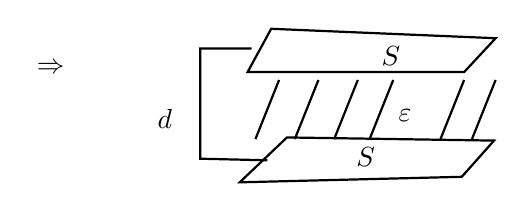
\begin{tikzpicture}[line width=0.8pt]
  \node at (-2.4,1.45) {$\Rightarrow$};
  \draw (0.1,1.4) -- (0.4,1.95) -- (3.25,1.83) -- (2.85,1.4) -- cycle;
  \draw (0,0) -- (0.6,0.57) -- (3.23,0.53) -- (2.82,0.07) -- cycle;
  \node at (1.92,1.6) {$S$};
  \node at (1.6,0.32) {$S$};
  \foreach \hx in {0.2,0.7,1.2,1.65,2.55,2.95} \draw (\hx,0.55) -- ++(0.3,0.75);
  \node at (2.1,0.85) {$\varepsilon$};
  \draw (0.15,1.7) -- (-0.5,1.7) -- (-0.5,0.3) -- (0.35,0.28);
  \node at (-0.95,0.8) {$d$};
\end{tikzpicture}
\end{center}

\[ C=\frac{\varepsilon\cdot S'}{d} \qquad\qquad \frac{(\mathrm{Farad}/\mathrm{m})\,(\mathrm{m}^{2})}{\mathrm{m}}=\mathrm{Farad} \]

Bir kürenin kapasitesi

\noindent
\begin{minipage}[c]{0.27\linewidth}
\centering
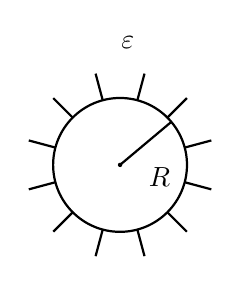
\begin{tikzpicture}[line width=0.8pt]
  \draw (0,0) circle (0.85);
  \fill (0,0) circle (0.8pt);
  \draw (0,0) -- (40:0.85);
  \node at (0.5,-0.15) {$R$};
  \foreach \a in {15,45,75,105,135,165,195,225,255,285,315,345} \draw (\a:0.85) -- (\a:1.2);
  \node at (0.1,1.55) {$\varepsilon$};
\end{tikzpicture}
\end{minipage}\hfill
\begin{minipage}[c]{0.70\linewidth}
\[ C=4\pi\varepsilon R \]
\[ V=\frac{V_s\cdot R}{r}=V_s\,\Phi\ \Rightarrow\ \Phi=\frac{R}{r} \]
\end{minipage}

\begin{flushright}
$dS=r^{2}\sin\theta\,d\theta\,d\varphi$
\end{flushright}

\begin{align*}
C &= -\varepsilon\int_{S_R}\frac{-R}{r^{2}} \\
&= C\,\varepsilon R\int_{\theta=0}^{\pi}\int_{\varphi=0}^{2\pi}\sin\theta\,d\theta\,d\varphi\qquad\text{\footnotemark}
\end{align*}
\footnotetext{Claude notu: baştaki $C$ muhtemelen fazla; sonuç $=4\pi\varepsilon R$.}
\[ =4\pi\varepsilon R \]

silindir için
\begin{gather*}
V=A\ln\rho \\
V=A\ln R=V_s\ \Rightarrow\ A=\frac{V_s}{\ln R}
\end{gather*}
\[ \Rightarrow\ V=\frac{V_s}{\ln R}\,\ln\rho=V_s\,\Phi\ \Rightarrow\ \Phi=\frac{\ln\rho}{\ln R} \]

$dn=d\rho$
\[ =-\varepsilon\int_{S'}\frac{\partial\Phi}{\partial n}\,dS=-\varepsilon\int\frac{\ln\rho}{\ln R}\,\underbrace{\rho\,d\varphi\,dz}_{dS}\qquad\text{\footnotemark} \]
\footnotetext{Claude notu: $\dfrac{\partial\Phi}{\partial\rho}=\dfrac{1}{\rho\,\ln R}$ olmalı (bir sonraki satırla tutarlı).}
\[ =-\varepsilon\int_{\varphi=0}^{2\pi}\int_{0}^{\ell}\frac{1}{\ln R}\,\frac{1}{\rho}\,\rho\,d\varphi\,dz=\frac{-\varepsilon}{\ln R}\,2\pi\ell \]

\sayfa{9}
\[ =\frac{2\pi\varepsilon\ell}{-\ln R}=\frac{2\pi\varepsilon\ell}{\ln(1/R)} \]

\noindent
\begin{minipage}[c]{0.40\linewidth}
\centering
\begin{circuitikz}[line width=0.7pt]
  \draw (0,0) to[C] (2.4,0);
  \draw (0,1.1) to[C] (2.4,1.1);
  \draw (0,2.2) to[C] (2.4,2.2);
  \draw (0,0) -- (0,2.2);
  \draw (2.4,0) -- (2.4,2.2);
\end{circuitikz}
\end{minipage}\hfill
\begin{minipage}[c]{0.56\linewidth}
\[ C=C_1+C_2+C_3 \]
\end{minipage}

\end{document}
